%% Copernicus Publications Manuscript Preparation Template for LaTeX Submissions
%% ---------------------------------
%% This template should be used for copernicus.cls
%% The class file and some style files are bundled in the Copernicus Latex Package, which can be downloaded from the different journal webpages.
%% For further assistance please contact Copernicus Publications at: production@copernicus.org
%% https://publications.copernicus.org/for_authors/manuscript_preparation.html
%% Please use the following documentclass and journal abbreviations for preprints and final revised papers.

%% 2-column papers and preprints
\documentclass[wes, manuscript]{copernicus}
%% Journal abbreviations (please use the same for preprints and final revised papers)

%% \usepackage commands included in the copernicus.cls:
%\usepackage[german, english]{babel}
%\usepackage{tabularx}
%\usepackage{cancel}
%\usepackage{multirow}
%\usepackage{supertabular}
%\usepackage{algorithmic}
%\usepackage{algorithm}
%\usepackage{amsthm}
%\usepackage{float}
%\usepackage{subfig}
%\usepackage{rotating}
\usepackage{booktabs}

\begin{document}

\title{Estimating offshore wind farm insta installation performance with satellite data}

% \Author[affil]{given_name}{surname}

\Author[1,3]{Aljoscha}{Sander}
% \Author[2]{Christian}{Backe}
\Author[1]{Eize}{Stamhuis}
\Author[4]{Albert}{Baars}

\affil[1]{University of Groningen, Groningen, The Netherlands}
% \affil[2]{German Research Center for Artificial Intelligence (DFKI), Bremen, Germany}
\affil[3]{University of Bremen, Bremen, Germany}
\affil[4]{University of Applied Sciences Bremen, Bremen, Germany}

%% The [] brackets identify the author with the corresponding affiliation. 1, 2, 3, etc. should be inserted.
%% If an author is deceased, please mark the respective author name(s) with a dagger, e.g. "\Author[2,$\dag$]{Anton}{Smith}", and add a further "\affil[$\dag$]{deceased, 1 July 2019}".
%% If authors contributed equally, please mark the respective author names with an asterisk, e.g. "\Author[2,*]{Anton}{Smith}" and "\Author[3,*]{Bradley}{Miller}" and add a further affiliation: "\affil[*]{These authors contributed equally to this work.}".

\correspondence{A.S. (aljoscha.sander@rug.nl)}
\runningtitle{Performance of Offshore Wind Farm Installations}
\runningauthor{Aljoscha Sander}


\received{}
\pubdiscuss{} %% only important for two-stage journals
\revised{}
\accepted{}
\published{}

%% These dates will be inserted by Copernicus Publications during the typesetting process.


\firstpage{1}
\maketitle

\begin{abstract}

\begin{itemize}

    \item Offshore wind maturing, installations are a massive challenge
    \item Little public data on offshore wind farm installation performance available
    \item Offshore Wind Farm Installation massively influenced by weather limits
    \item Combining Automatic Identification System (AIS), ERA5 and public wind farm data allows to assess performance of
offshore wind farm installation as a function of metocean data, location, wind turbine type and installation vessel

\end{itemize}

\end{abstract}


\copyrightstatement{TEXT} %% This section is optional and can be used for copyright transfers.


\introduction  %% \introduction[modified heading if necessary]

With 5,795 offshore wind turbines operational in Europe alone (June 2022),
offshore wind has become a major source of electricity in several countries, 
and more than 20 years of installing offshore wind farms has led to a significant
amount of learning in the industry. While a great deal of scientific 
literature is available on wind turbine design and operations, the body of 
literature dealing with offshore wind farm installations is 
comparatively small, even though installing wind turbines offshore imposes a
complex and thus scientifically interesting problem.

The installation of an offshore wind farm is by no means an easy undertaking: 
metocean conditions must be within narrow limits to allow save operations. 
Specialized equipment, vessels, and crews are required. The continuously 
increasing size of turbines, as well as increasing water depths, and new locations 
where little experience is available, add to the risks associated with installations. 
Unforeseen downtimes are costly and put additional strain on already difficult operations. 

In this study, we investigate how metocean conditions correlate with offshore wind farm 
installation times. We compile a statistical overview of offshore wind farm installations: 
from satellite data, we extract correlations between turbine size, wind farm locations, 
installation vessels and installation duration with metocean conditions during the installation process. Finally, we extract the observed metocean limits for turbine sizes, manufacturers, vessels, and locations

\section{Material and Methods}

\subsection{Vessel tracks}

\paragraph{Data acquisition and pre-processing}

To reliably extract installation times for as many offshore wind farms as possible, 
we acquired hourly \textit{Automatic Identification System} (AIS) vessel data from a 
data broker. The AIS data includes 9 offshore wind installation vessels over a 
period of 11 years (see \autoref{tab:ais}).  

\begin{table}[]
    \caption{AIS vessel data used in this study.}
    \centering
    \begin{tabular}{c c c}
        MMSI & Name & Data time range \\
        \hline
        218389000 & Thor & 2010 - 2021 \\
        218657000 & Vole au Vent & 2013 - 2021 \\
        219019002 & Sea Challenger & 2013 - 2021 \\
        229044000 & Brave Tern & 2012 - 2021 \\
        229080000 & Bold Tern & 2013 - 2021 \\
        235090598 & Blue Tern & 2015 - 2021 \\
        245179000 & Aeolus &  2010 - 2021 \\
        245924000 & MPI Adventure & 2010 - 2021 \\
        246777000 & MPI Resolution & 2010 - 2021 \\
    \end{tabular}
    \label{tab:ais}
\end{table}

Each AIS vessel record includes latitude, longitude, speed, heading, course and a 
timestamp for a given vessel.

\paragraph{Clustering vessel tracks to extract wind farms}
To extract installation times per turbine per offshore 
wind farm, we preselected vessel records where the speed of the vessel was 0 and further 
removed records where the vessel was close to shore or in port. The vessel records were 
then automatically clustered using the DBSCAN algorithm as implemented in the 
scikit-learn python package. 
\paragraph{Clustering wind farms to extract single turbines}
To yield vessel records corresponding to single turbine installations, 
each wind farm cluster was clustered again with the DBSCAN algorithm, yielding vessel 
records corresponding to individual turbines. Only turbine locations where at least two 
vessel records were available were kept for further analysis.
Installation times per turbine were then calculated by assuming, that the first available 
AIS vessel record corresponds to the beginning of turbine installation activities and the 
last AIS record marks the end of installation activities.

\subsection{Wind farms}
These clusters were then cross-referenced with the 
locations of offshore wind farms to select vessel records within a given radius of a 
known wind farm. 

\subsection{Metocean data}
Based on the time stamps of the AIS records per turbine, ERA5 metocean data was 
requested for the wind farm location. ERA5 data includes wind speed and wind direction at several 
altitudes, wave direction, wave period and significant wave height. For each wind farm, 
metadata such as wind turbine model, rated power and foundation type were collected, 
and all data was combined into a SQLite database. The database will be made available 
to the public once analysis has been completed. 

\clearpage
\newpage

\section{Results and Discussion}

\begin{table}[ht]
    \caption[]{Overview of detected wind farms and number of extracted wind turbines per wind farm}
    \centering
    \input{windfarms.txt}
    \label{tab:installations}
\end{table}

\clearpage
\newpage

\begin{figure}[h]
    \centering
    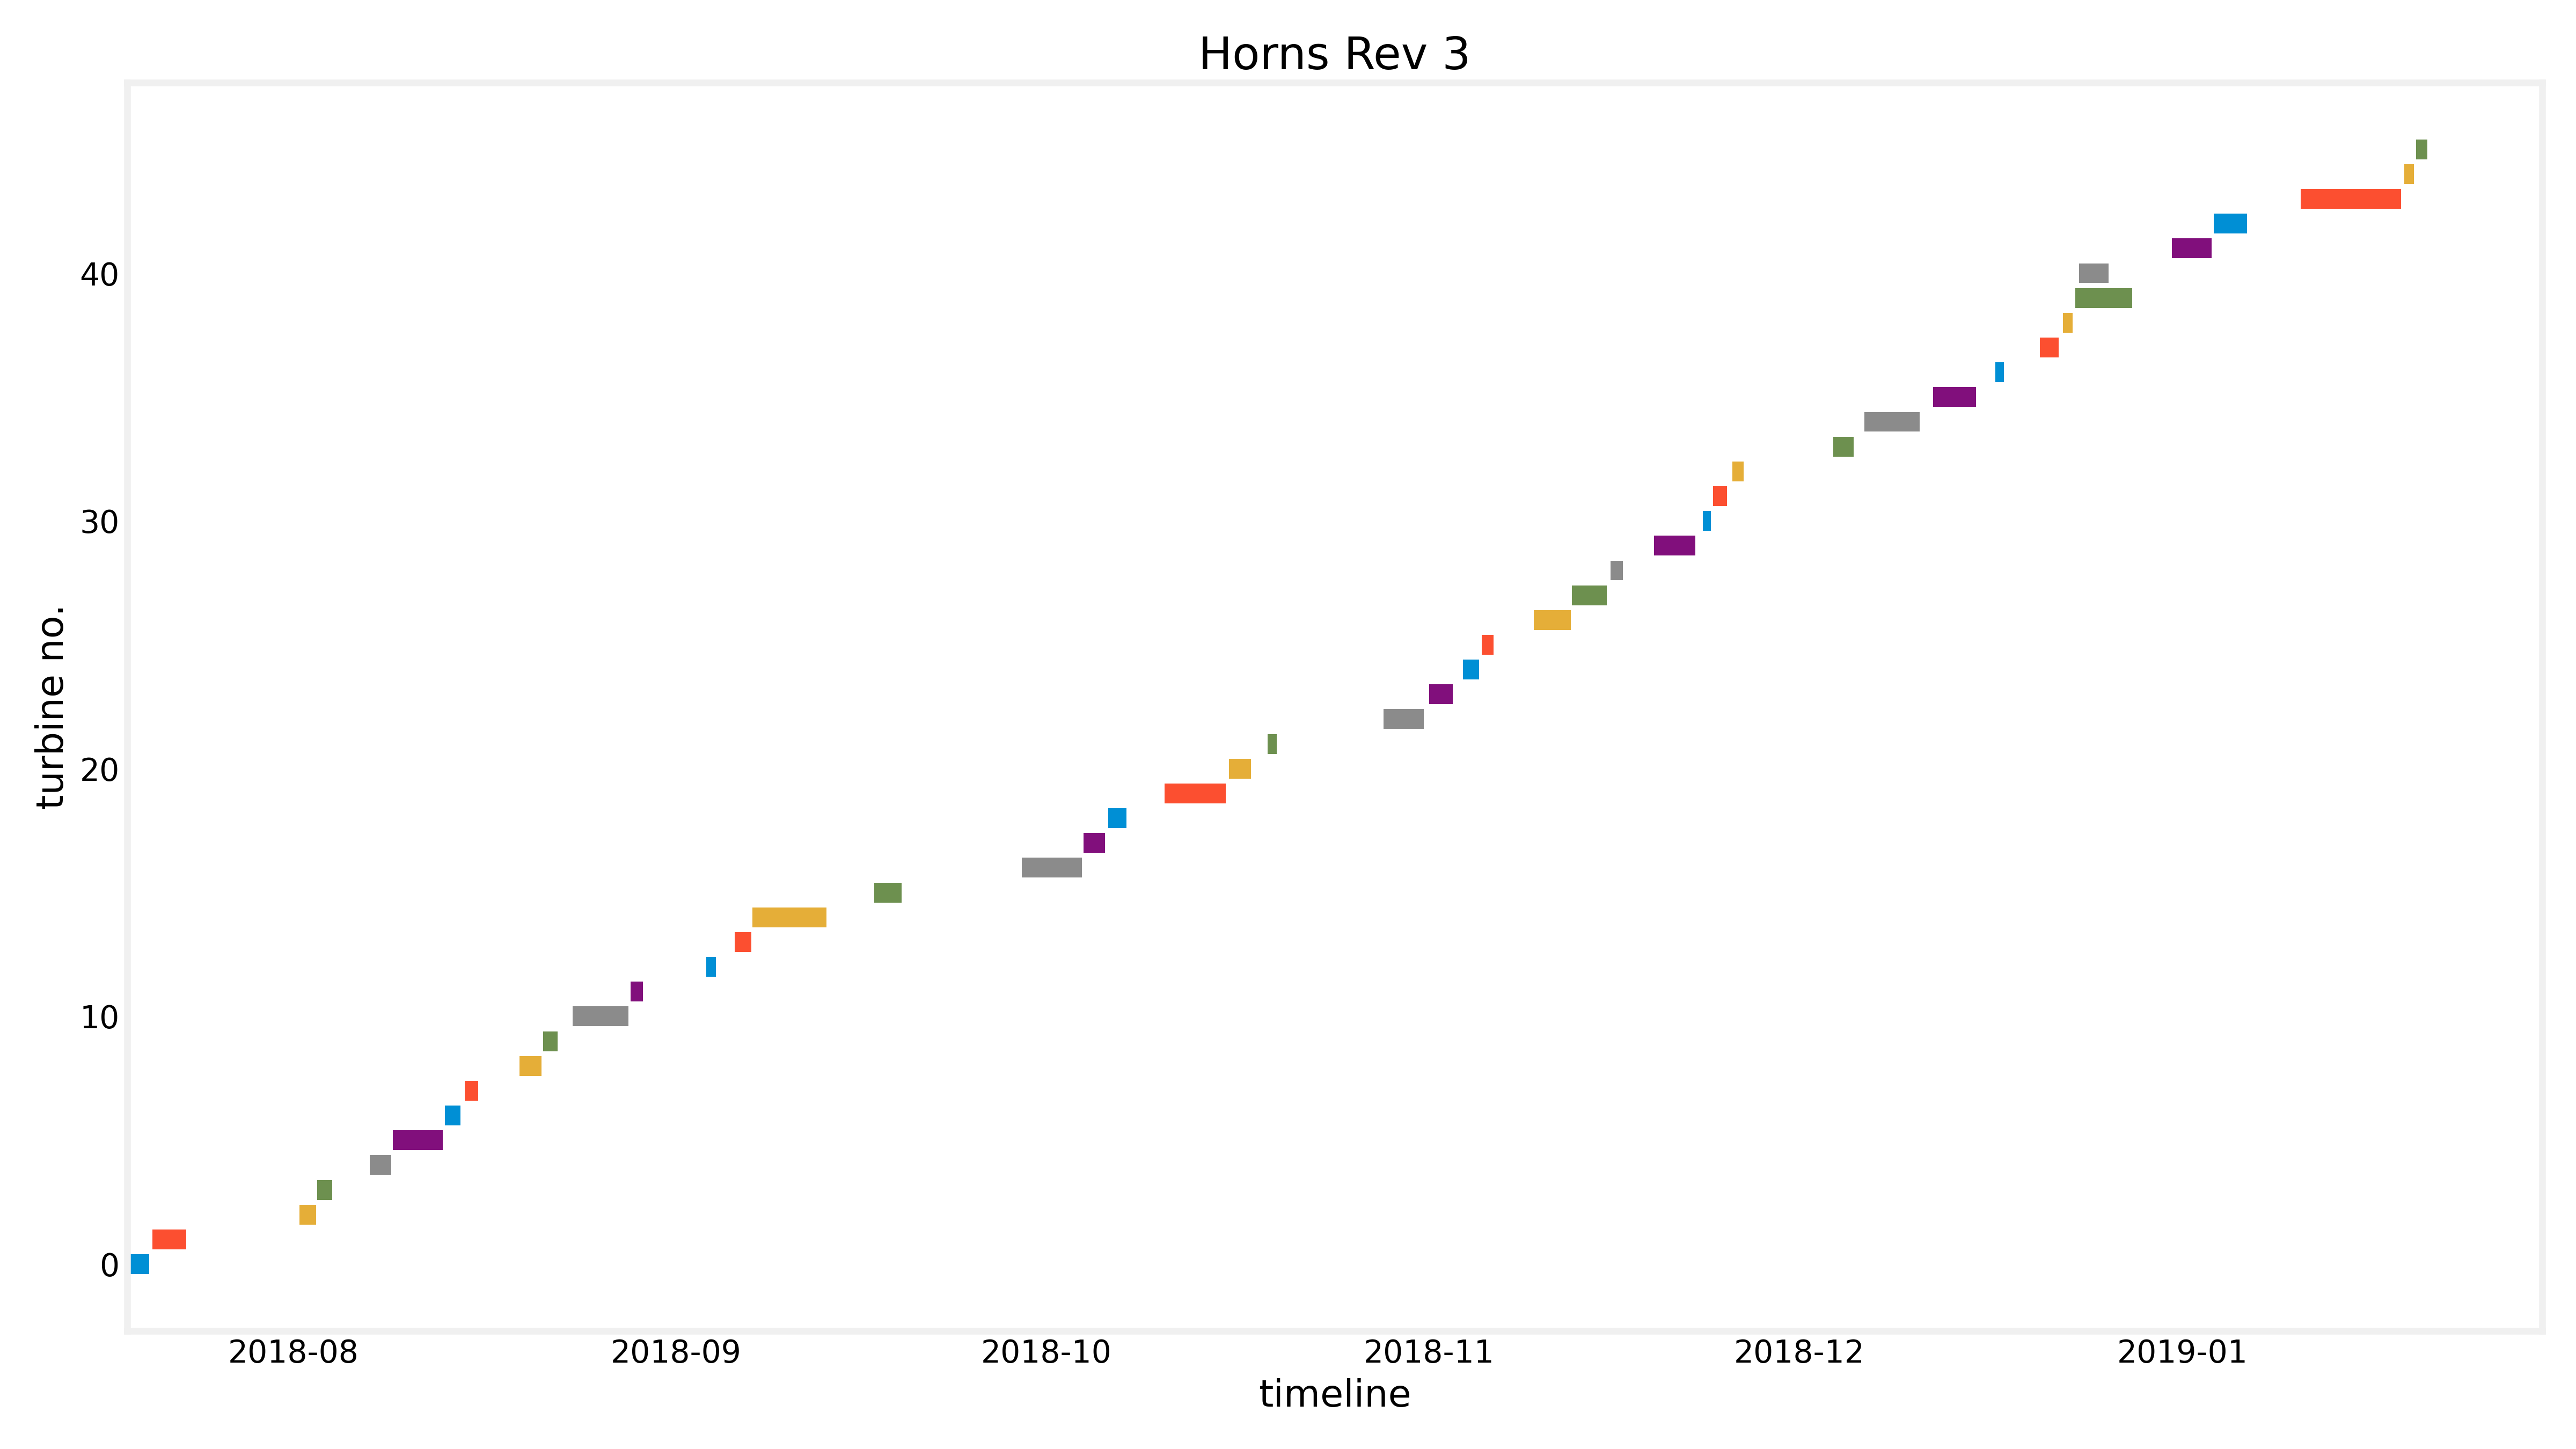
\includegraphics[width=\textwidth]{figures/gantt/Horns Rev 3.png}
    \caption{duration distribution}
    \label{fig:wind}
\end{figure}
\begin{figure}[h]
    \centering
    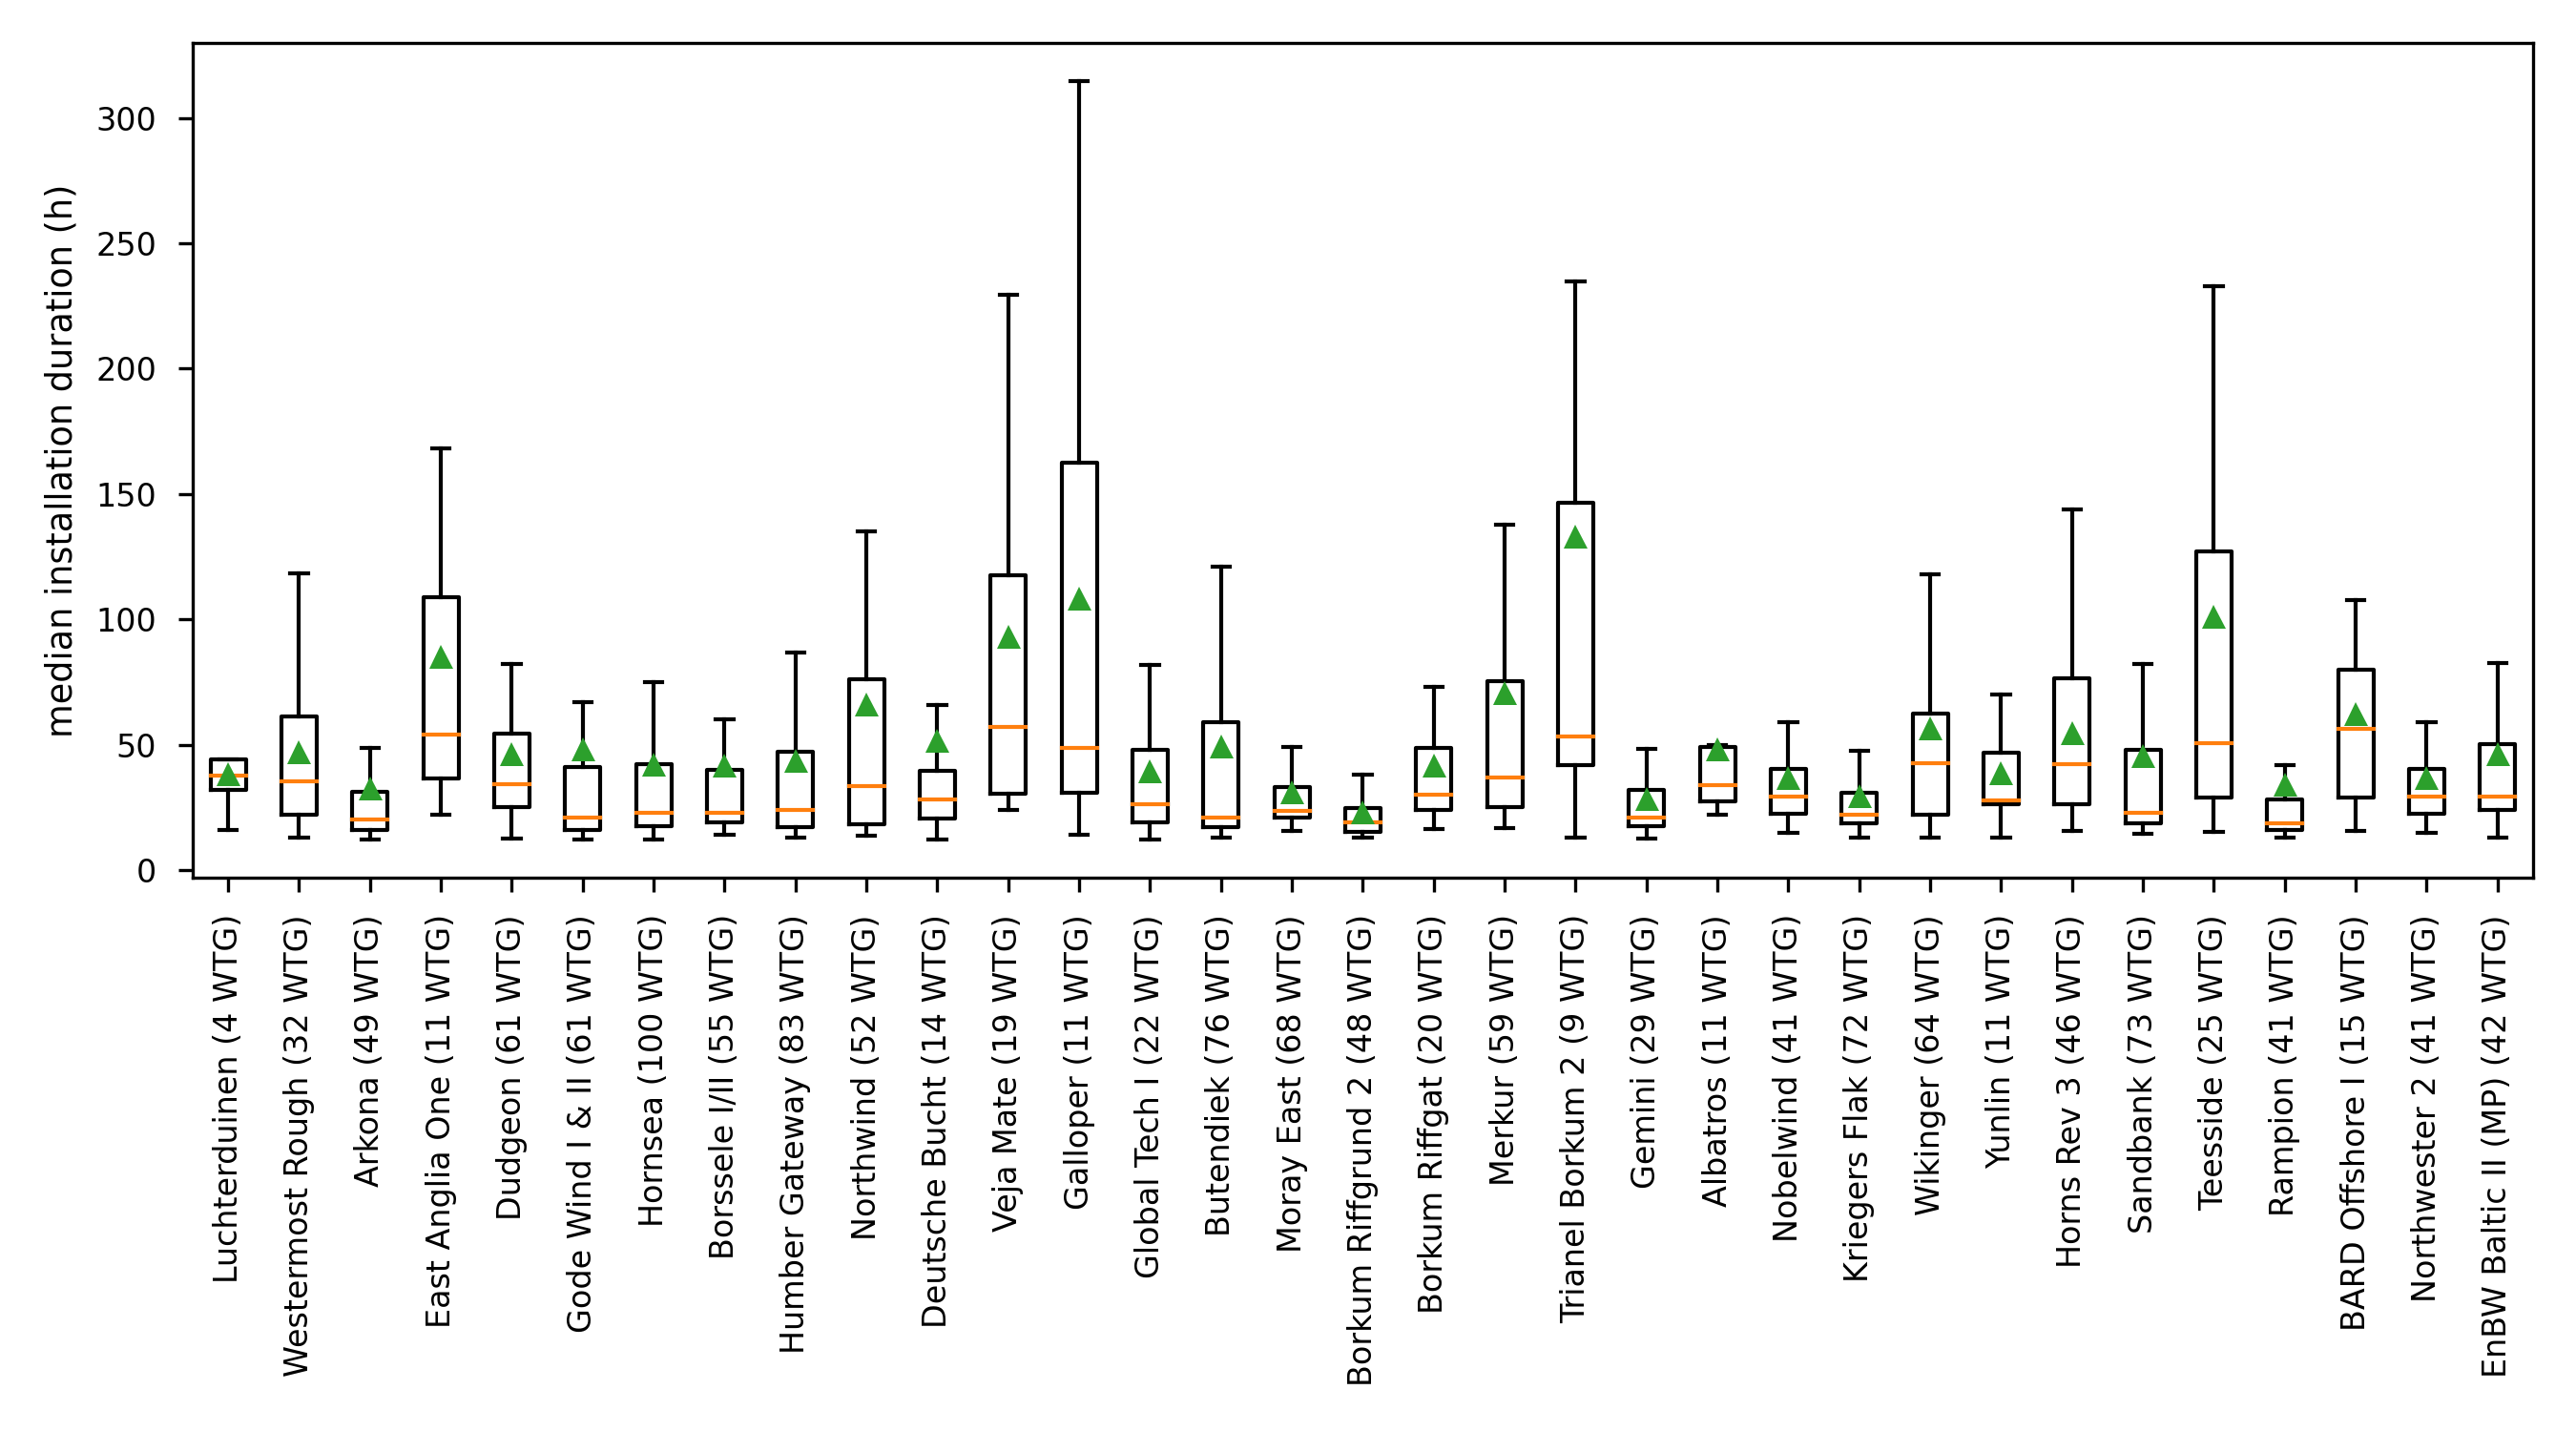
\includegraphics[width=\textwidth]{figures/installations-overview.png}
    \caption{Overview of installation data}
    \label{fig:overview}
\end{figure}

\begin{figure}[h]
    \centering
    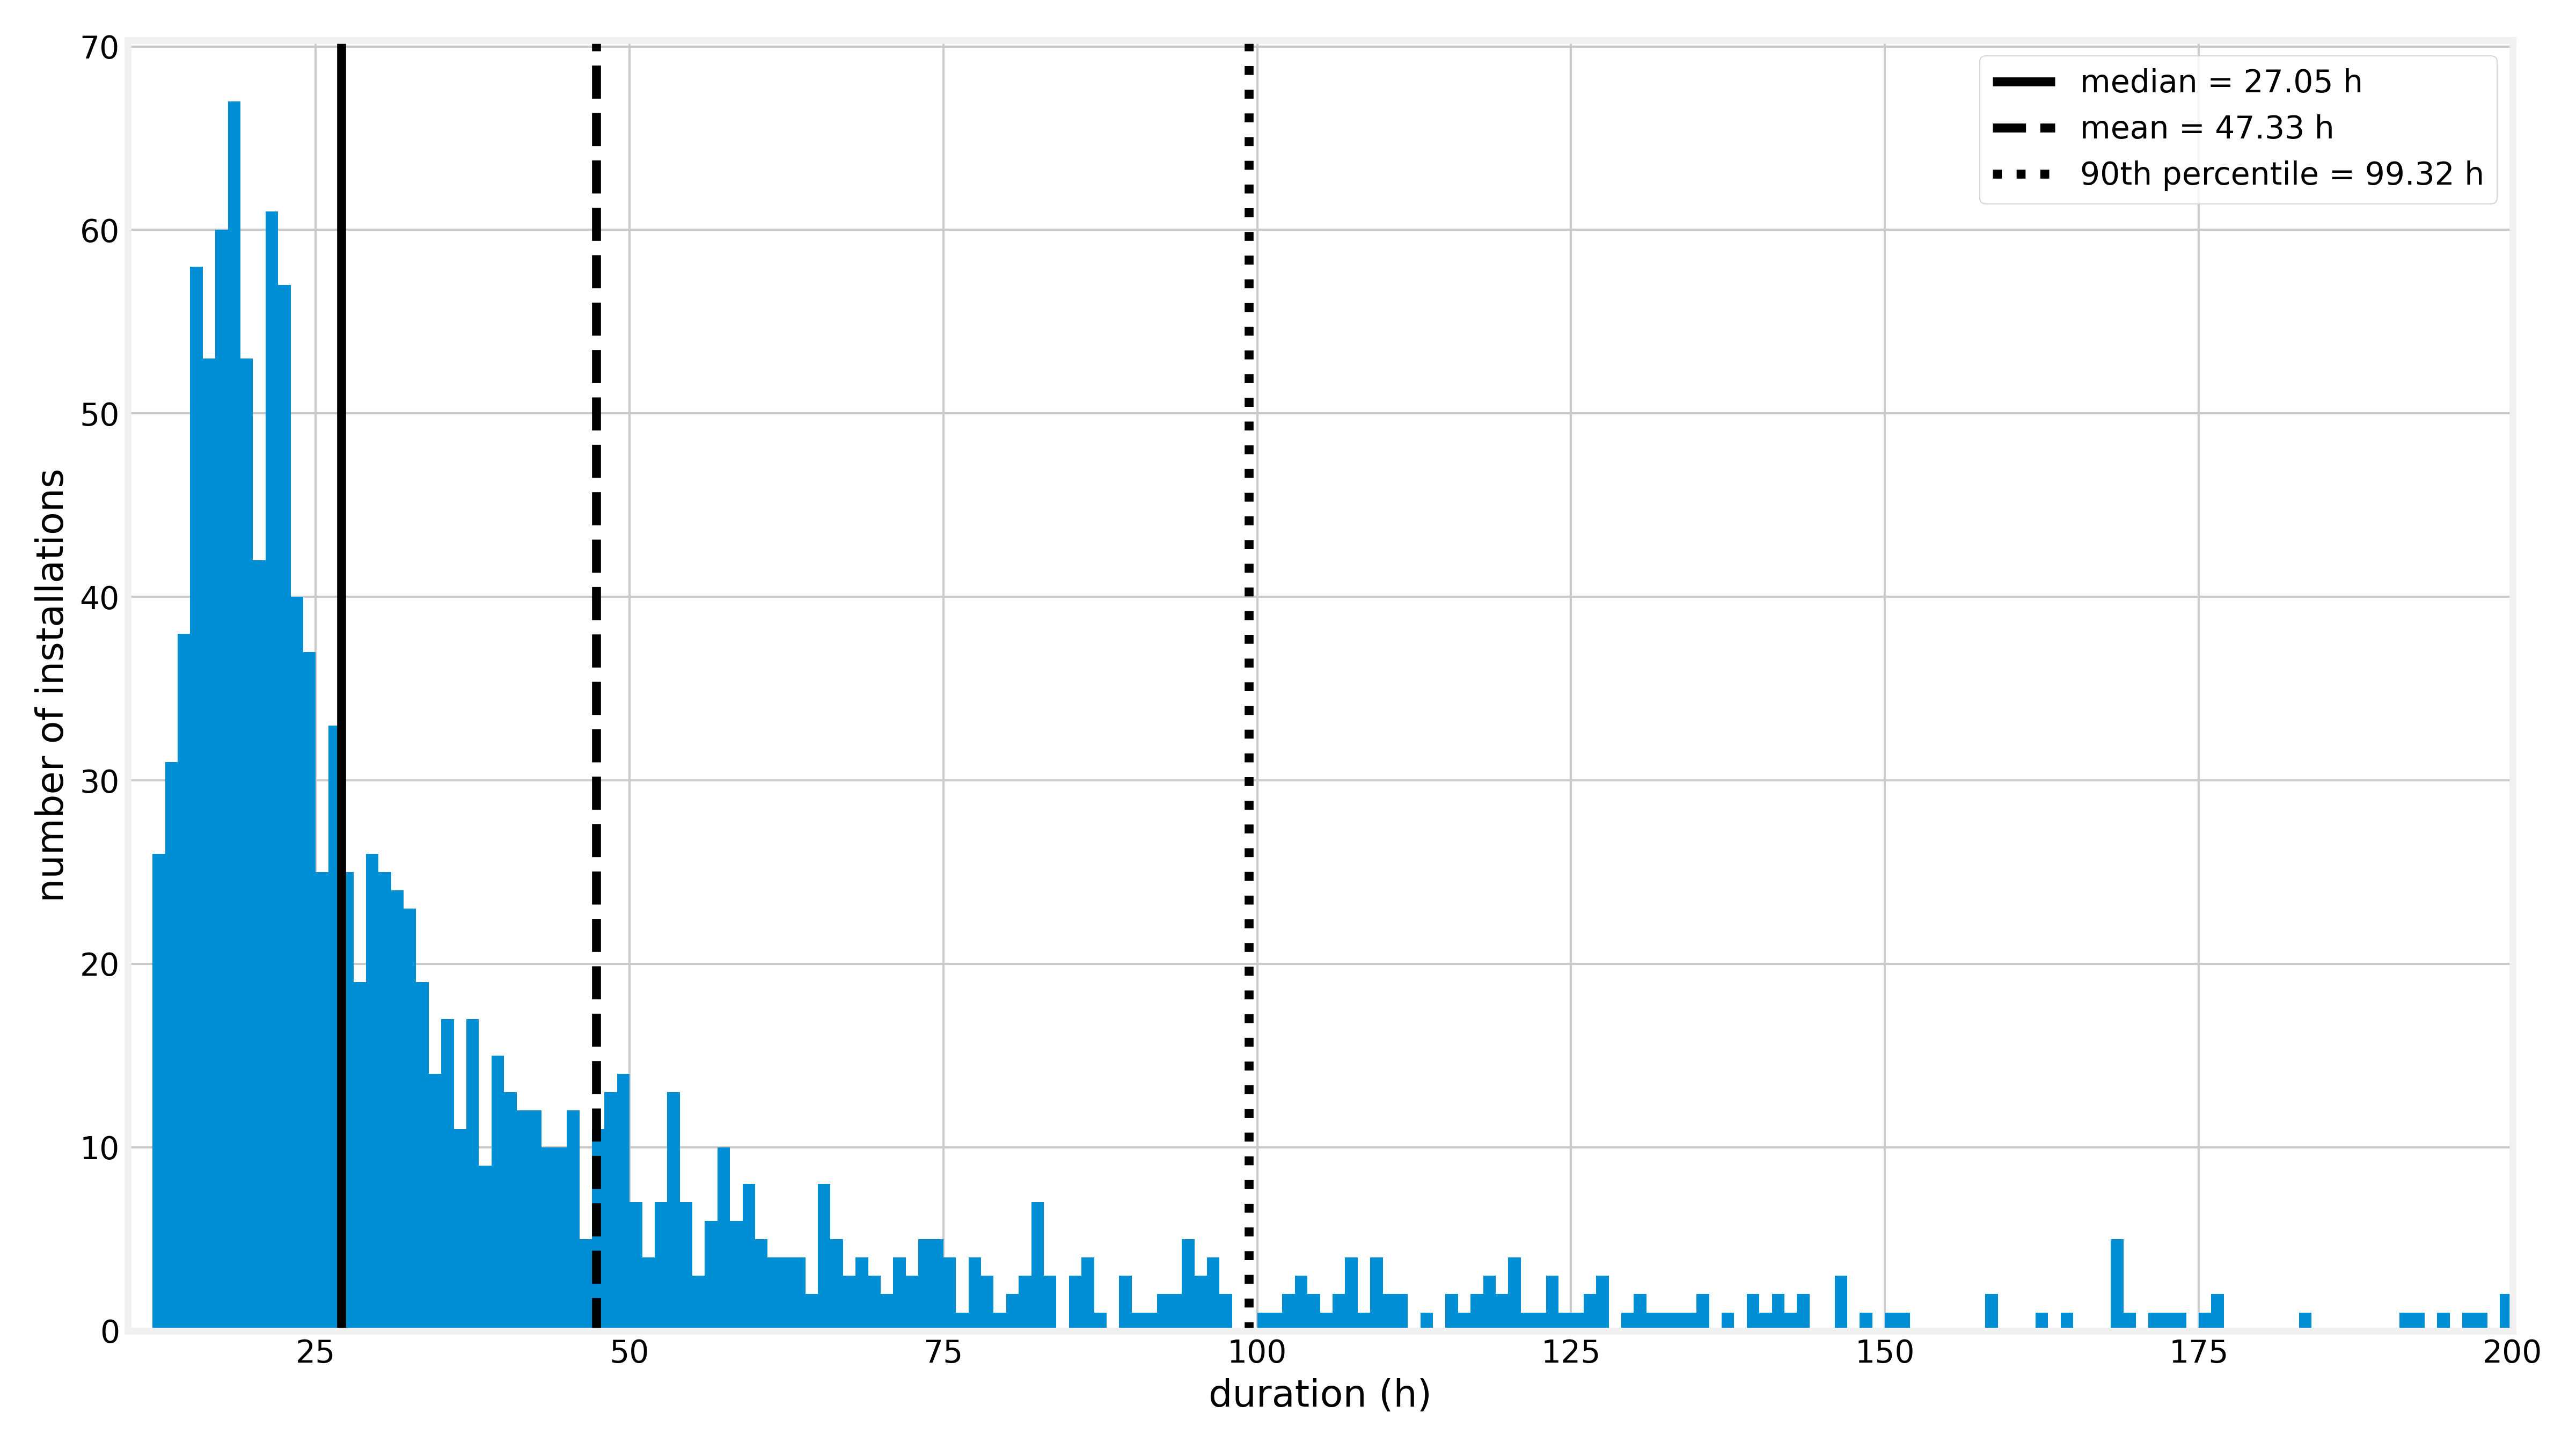
\includegraphics[width=\textwidth]{figures/duration-distribution.png}
    \caption{duration distribution}
    \label{fig:distribution}
\end{figure}

\begin{figure}[h]
    \centering
    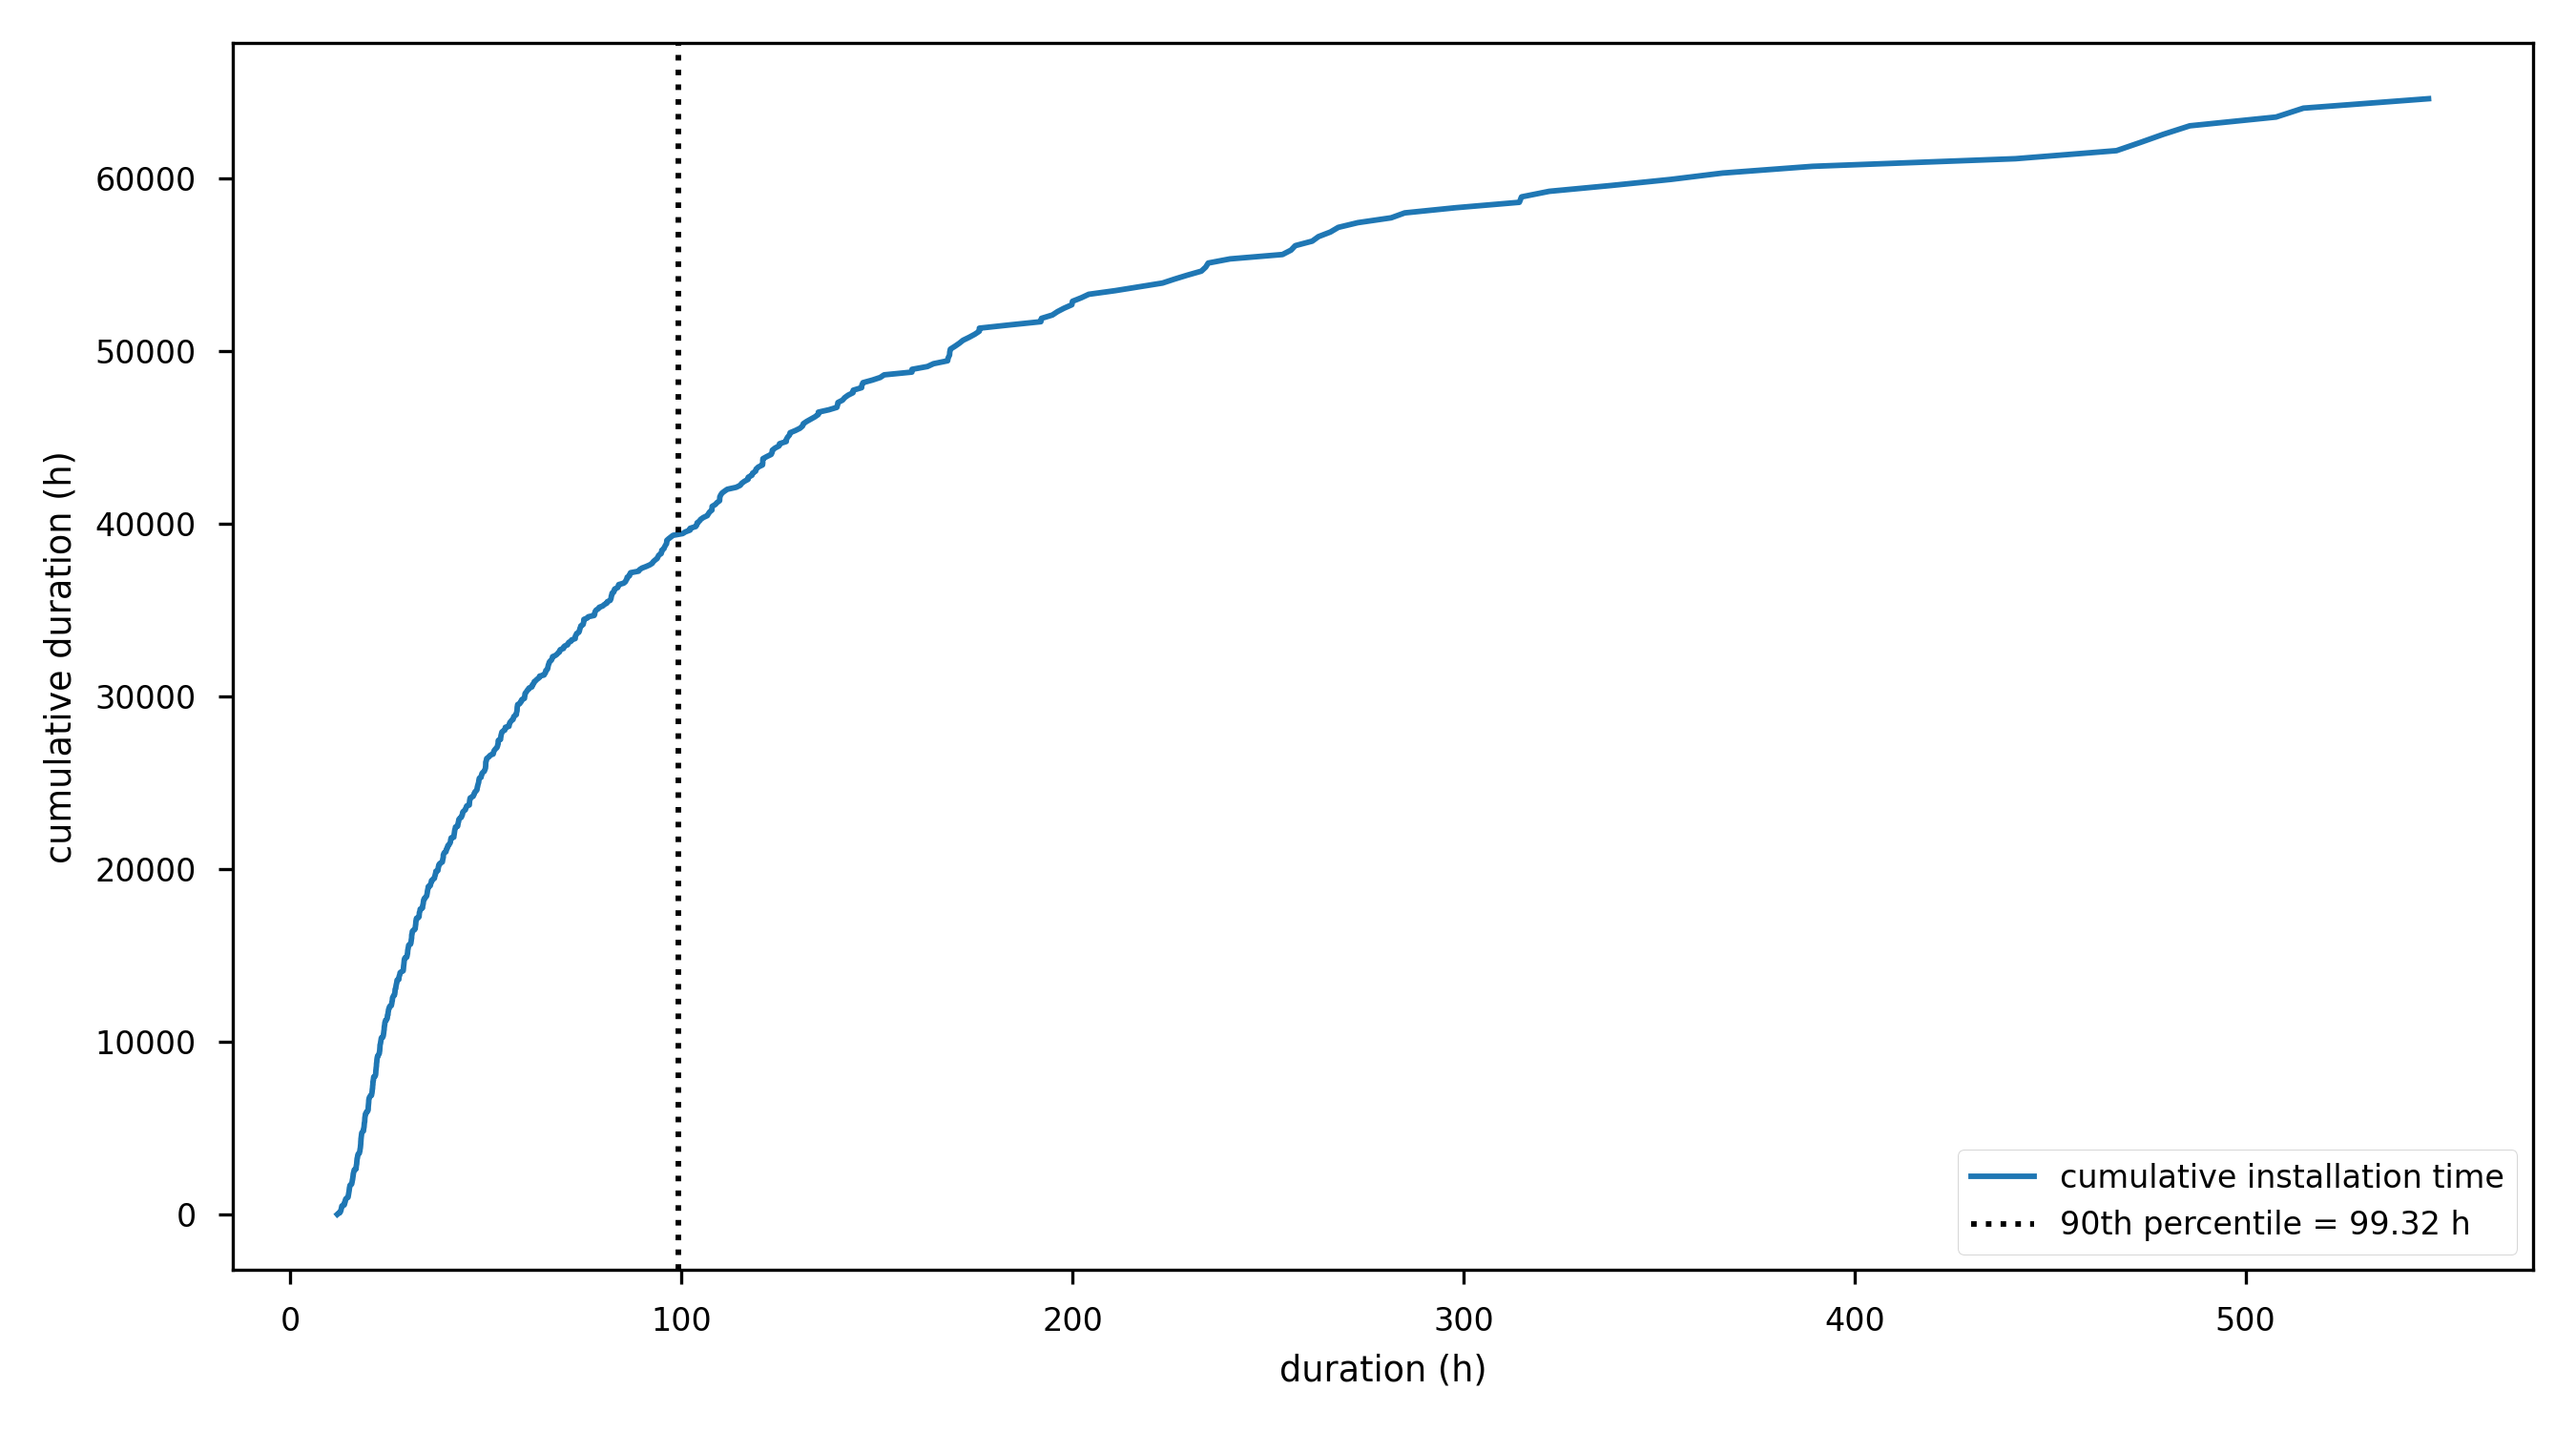
\includegraphics[width=\textwidth]{figures/cumulative-duration.png}
    \caption{duration distribution}
    \label{fig:cumsum}
\end{figure}

\begin{figure}[h]
    \centering
    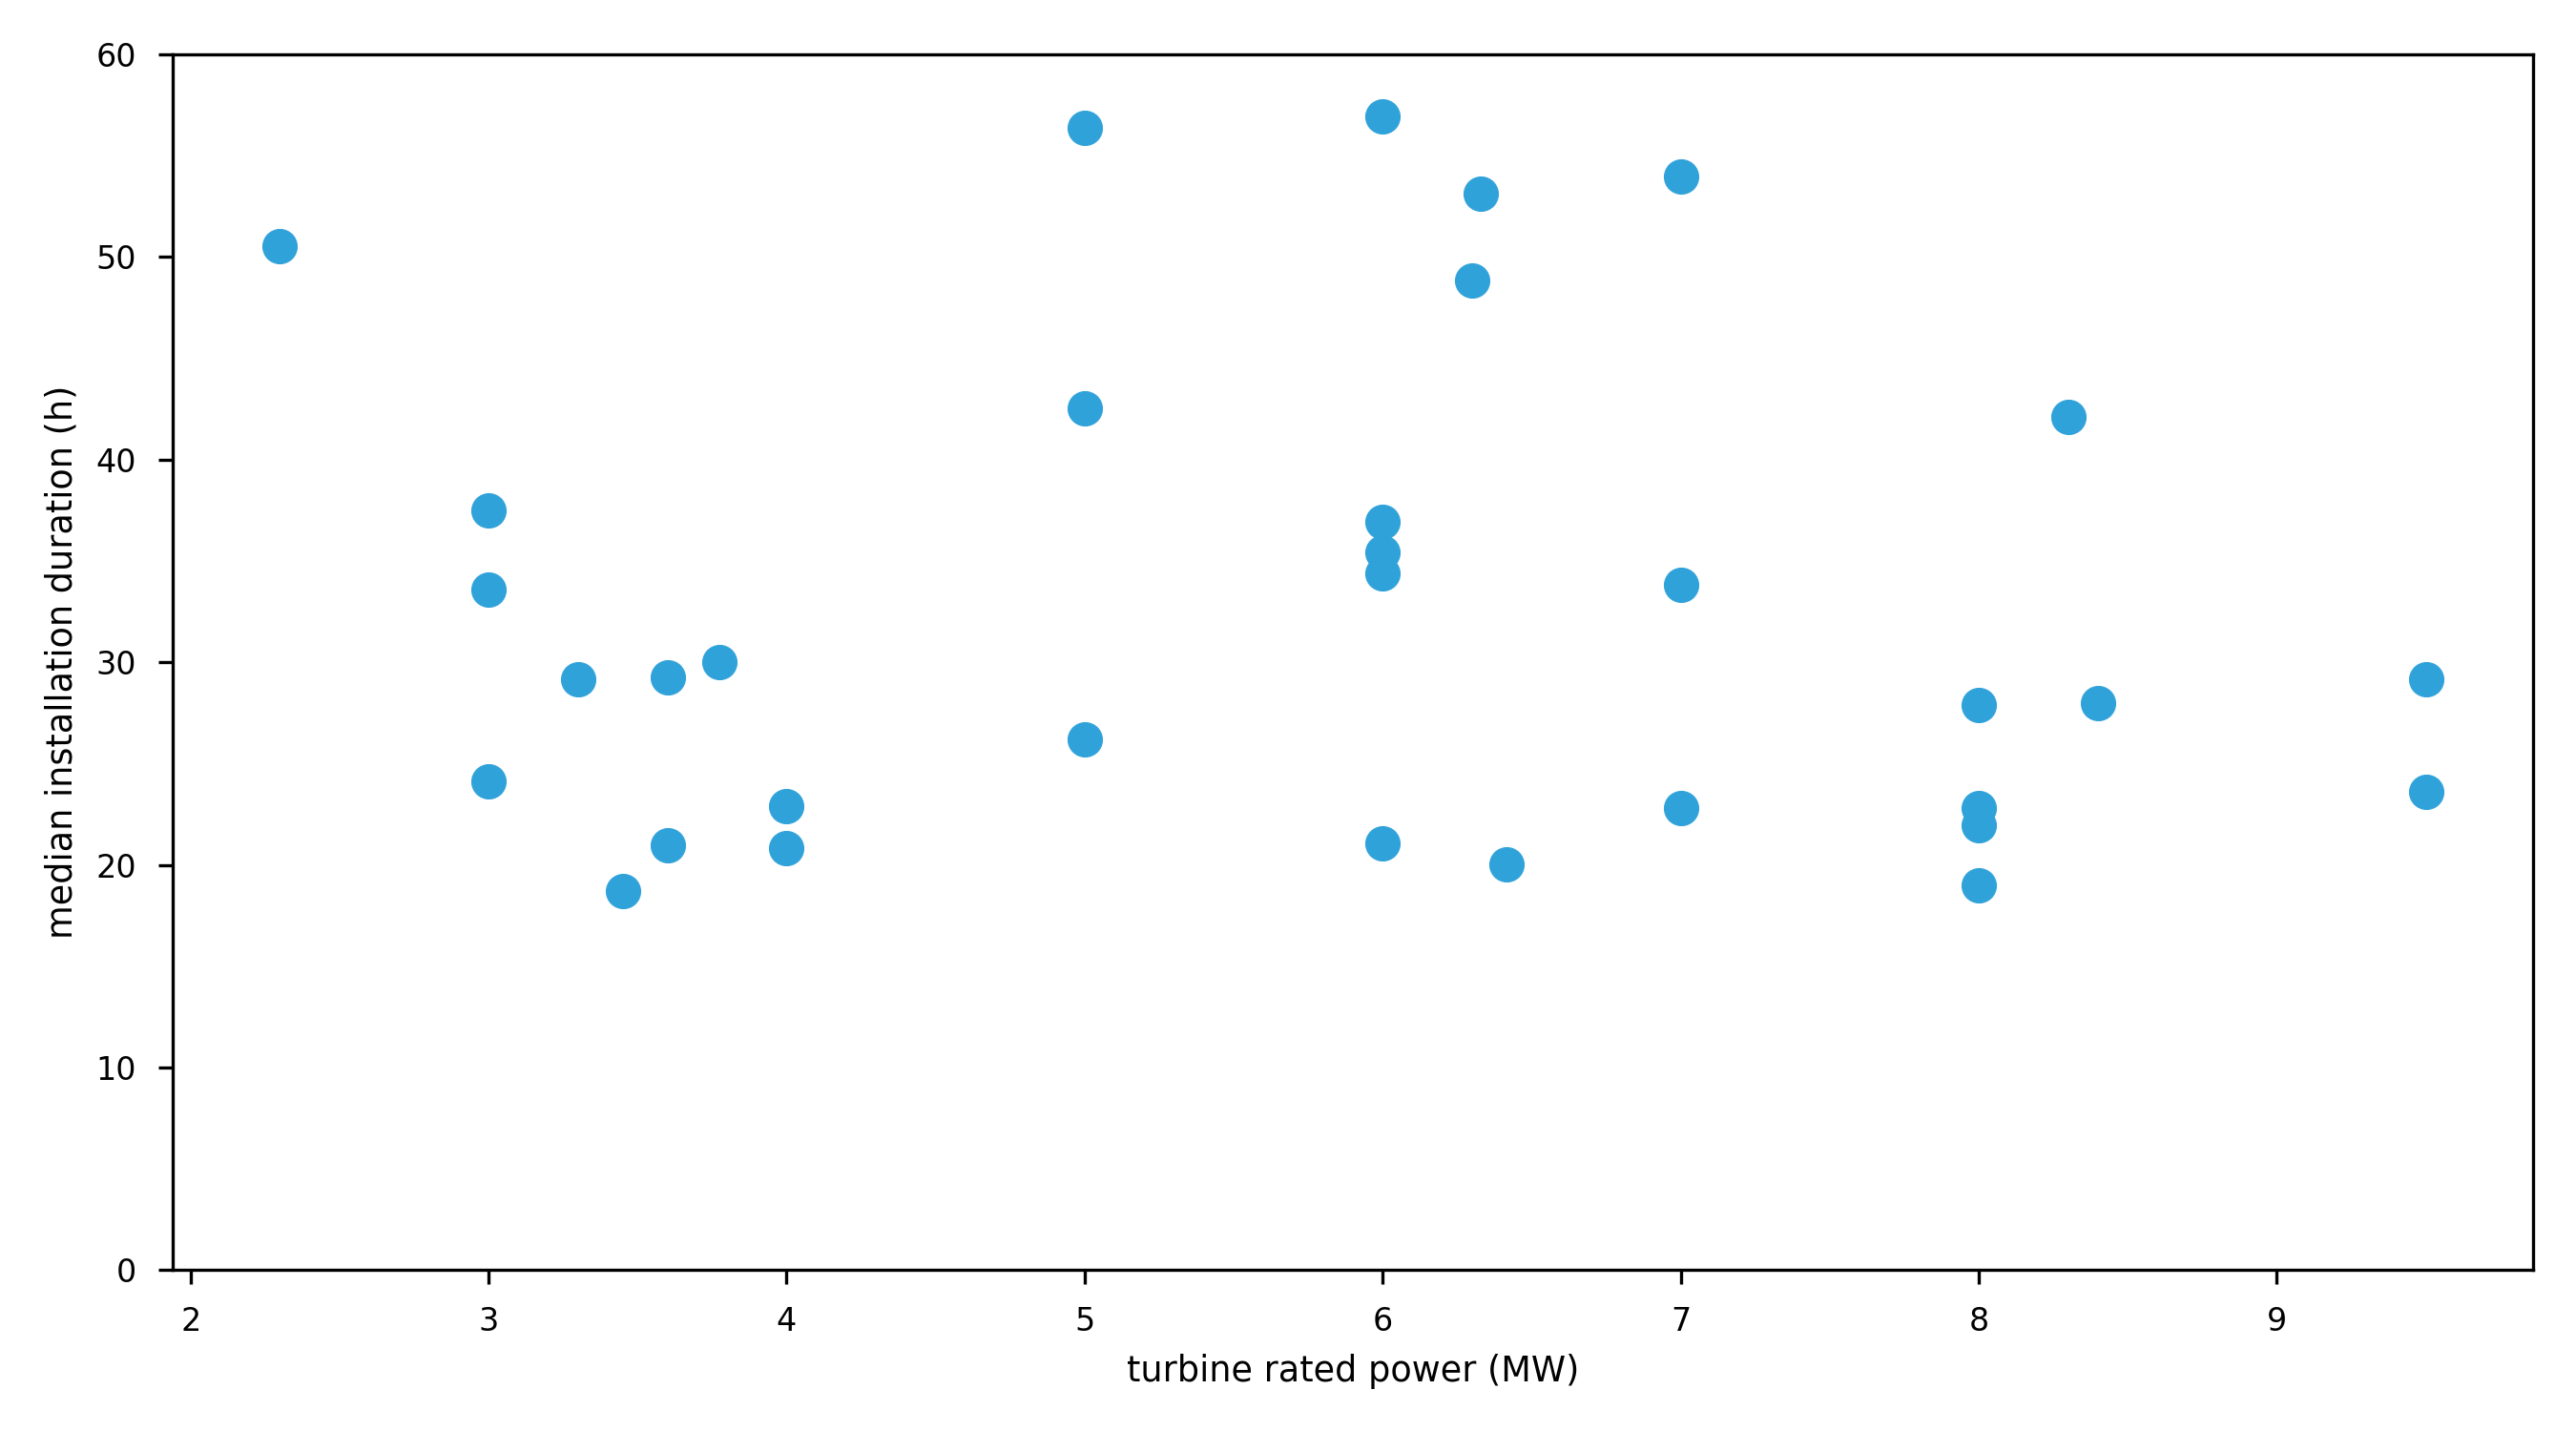
\includegraphics[width=\textwidth]{figures/durations-rated-power.png}
    \caption{duration distribution}
    \label{fig:size}
\end{figure}
\conclusions  %% \conclusions[modified heading if necessary]


\clearpage
\newpage

\conclusions  %% \conclusions[modified heading if necessary]



%% The following commands are for the statements about the availability of data sets and/or software code corresponding to the manuscript.
%% It is strongly recommended to make use of these sections in case data sets and/or software code have been part of your research the article is based on.


\codedataavailability{All code related to the present publication is available
on github under creative-commons licence: 
\url{https://github.com/k323r/2022_WES_offshore-wind-installation}}


\sampleavailability{TEXT} %% use this section when having geoscientific samples available


\appendix
\section{}    %% Appendix A

\subsection{}     %% Appendix A1, A2, etc.


\noappendix       %% use this to mark the end of the appendix section. Otherwise the figures might be numbered incorrectly (e.g. 10 instead of 1).

%% Regarding figures and tables in appendices, the following two options are possible depending on your general handling of figures and tables in the manuscript environment:

%% Option 1: If you sorted all figures and tables into the sections of the text, please also sort the appendix figures and appendix tables into the respective appendix sections.
%% They will be correctly named automatically.

%% Option 2: If you put all figures after the reference list, please insert appendix tables and figures after the normal tables and figures.
%% To rename them correctly to A1, A2, etc., please add the following commands in front of them:

\appendixfigures  %% needs to be added in front of appendix figures

\appendixtables   %% needs to be added in front of appendix tables

%% Please add \clearpage between each table and/or figure. Further guidelines on figures and tables can be found below.


\authorcontribution{TEXT} %% this section is mandatory

\competinginterests{TEXT} %% this section is mandatory even if you declare that no competing interests are present

\disclaimer{TEXT} %% optional section

\begin{acknowledgements}
TEXT
\end{acknowledgements}




%% REFERENCES

%% The reference list is compiled as follows:

\begin{thebibliography}{}

\bibitem[AUTHOR(YEAR)]{LABEL1}
REFERENCE 1

\bibitem[AUTHOR(YEAR)]{LABEL2}
REFERENCE 2

\end{thebibliography}

%% Since the Copernicus LaTeX package includes the BibTeX style file copernicus.bst,
%% authors experienced with BibTeX only have to include the following two lines:
%%
%% \bibliographystyle{copernicus}
%% \bibliography{example.bib}
%%
%% URLs and DOIs can be entered in your BibTeX file as:
%%
%% URL = {http://www.xyz.org/~jones/idx_g.htm}
%% DOI = {10.5194/xyz}


%% LITERATURE CITATIONS
%%
%% command                        & example result
%% \citet{jones90}|               & Jones et al. (1990)
%% \citep{jones90}|               & (Jones et al., 1990)
%% \citep{jones90,jones93}|       & (Jones et al., 1990, 1993)
%% \citep[p.~32]{jones90}|        & (Jones et al., 1990, p.~32)
%% \citep[e.g.,][]{jones90}|      & (e.g., Jones et al., 1990)
%% \citep[e.g.,][p.~32]{jones90}| & (e.g., Jones et al., 1990, p.~32)
%% \citeauthor{jones90}|          & Jones et al.
%% \citeyear{jones90}|            & 1990



%% FIGURES

%% When figures and tables are placed at the end of the MS (article in one-column style), please add \clearpage
%% between bibliography and first table and/or figure as well as between each table and/or figure.

% The figure files should be labelled correctly with Arabic numerals (e.g. fig01.jpg, fig02.png).


%% ONE-COLUMN FIGURES

%%f
%\begin{figure}[t]
%\includegraphics[width=8.3cm]{FILE NAME}
%\caption{TEXT}
%\end{figure}
%
%%% TWO-COLUMN FIGURES
%
%%f
%\begin{figure*}[t]
%\includegraphics[width=12cm]{FILE NAME}
%\caption{TEXT}
%\end{figure*}
%
%
%%% TABLES
%%%
%%% The different columns must be seperated with a & command and should
%%% end with \\ to identify the column brake.
%
%%% ONE-COLUMN TABLE
%
%%t
%\begin{table}[t]
%\caption{TEXT}
%\begin{tabular}{column = lcr}
%\tophline
%
%\middlehline
%
%\bottomhline
%\end{tabular}
%\belowtable{} % Table Footnotes
%\end{table}
%
%%% TWO-COLUMN TABLE
%
%%t
%\begin{table*}[t]
%\caption{TEXT}
%\begin{tabular}{column = lcr}
%\tophline
%
%\middlehline
%
%\bottomhline
%\end{tabular}
%\belowtable{} % Table Footnotes
%\end{table*}
%
%%% LANDSCAPE TABLE
%
%%t
%\begin{sidewaystable*}[t]
%\caption{TEXT}
%\begin{tabular}{column = lcr}
%\tophline
%
%\middlehline
%
%\bottomhline
%\end{tabular}
%\belowtable{} % Table Footnotes
%\end{sidewaystable*}
%
%
%%% MATHEMATICAL EXPRESSIONS
%
%%% All papers typeset by Copernicus Publications follow the math typesetting regulations
%%% given by the IUPAC Green Book (IUPAC: Quantities, Units and Symbols in Physical Chemistry,
%%% 2nd Edn., Blackwell Science, available at: http://old.iupac.org/publications/books/gbook/green_book_2ed.pdf, 1993).
%%%
%%% Physical quantities/variables are typeset in italic font (t for time, T for Temperature)
%%% Indices which are not defined are typeset in italic font (x, y, z, a, b, c)
%%% Items/objects which are defined are typeset in roman font (Car A, Car B)
%%% Descriptions/specifications which are defined by itself are typeset in roman font (abs, rel, ref, tot, net, ice)
%%% Abbreviations from 2 letters are typeset in roman font (RH, LAI)
%%% Vectors are identified in bold italic font using \vec{x}
%%% Matrices are identified in bold roman font
%%% Multiplication signs are typeset using the LaTeX commands \times (for vector products, grids, and exponential notations) or \cdot
%%% The character * should not be applied as mutliplication sign
%
%
%%% EQUATIONS
%
%%% Single-row equation
%
%\begin{equation}
%
%\end{equation}
%
%%% Multiline equation
%
%\begin{align}
%& 3 + 5 = 8\\
%& 3 + 5 = 8\\
%& 3 + 5 = 8
%\end{align}
%
%
%%% MATRICES
%
%\begin{matrix}
%x & y & z\\
%x & y & z\\
%x & y & z\\
%\end{matrix}
%
%
%%% ALGORITHM
%
%\begin{algorithm}
%\caption{...}
%\label{a1}
%\begin{algorithmic}
%...
%\end{algorithmic}
%\end{algorithm}
%
%
%%% CHEMICAL FORMULAS AND REACTIONS
%
%%% For formulas embedded in the text, please use \chem{}
%
%%% The reaction environment creates labels including the letter R, i.e. (R1), (R2), etc.
%
%\begin{reaction}
%%% \rightarrow should be used for normal (one-way) chemical reactions
%%% \rightleftharpoons should be used for equilibria
%%% \leftrightarrow should be used for resonance structures
%\end{reaction}
%
%
%%% PHYSICAL UNITS
%%%
%%% Please use \unit{} and apply the exponential notation


\end{document}
